% !TEX encoding = UTF-8
% !TEX TS-program = pdflatex
% !TEX root = ../tesi.tex

%**************************************************************
\chapter{Integrazione di Amazon Rekognition}
\label{cap:rekognition}
%**************************************************************

In questo capitolo viene approfondito lo sviluppo e l'integrazione del sistema di image recognition all'interno dell'applicativo.\\

%**************************************************************

\section{Presentazione del problema}
MariBa è una piattaforma per il salvataggio dei risultati delle partite giocate dai dipendenti di \azienda durante le 
pause pranzo e caffè. \\
L'inizializzazione di una partita prevede l'inserimento dei nomi di tutti i giocatori, specificando anche la posizione (attacco o difesa) e le squadre nel caso del biliardino. Questo procedimento di inserimento dei dati iniziali
risultava laborioso ed è stata quindi espressa la necessità di velocizzare tale procedura. \\
L'idea è quella di scattare una foto ai giocatori partecipanti in modo tale che l'applicazione li riconosca in modo automatico.

\section{Progettazione}
In questa sezione vengono descritti l'architettura ed il funzionamento del sistema di riconoscimento facciale implementato. \\
Successivamente viene presentato e approfondito il design dell'applicazione web dopo l'integrazione.

	\subsection{Architettura}
	 Il micro-servizio sviluppato fa uso di diverse tecnologie rese disponibili da \gls{AWS}: 
	 \begin{itemize}
	 	\item \emph{Amazon Rekognition};
	 	\item \emph{Amazon S3};
	 	\item \emph{AWS Lambda}
	 \end{itemize}
 	Nei prossimi paragrafi vengono descritte nel dettaglio tali tecnologie, il loro ruolo all'interno dell'applicativo e come esse collaborino tra loro per il raggiungimento dell'obiettivo.
	
	\subsubsection{Amazon Rekognition} \label{subsec:rekognition}
	
	\emph{Amazon Rekognition} è un software \emph{cloud-based} che mette a disposizione capacità di visione artificiale pre-addestrate e personalizzabili per estrarre informazioni dettagliate da immagini e video. Nel caso del progetto è stato utilizzato per indicizzare le facce e permetterne quindi il riconoscimento. In particolare, tutte le facce sono state salvate all'interno di una raccolta (\emph{collection}) ed a ciascuna di esse è stato assegnato un ID univoco (\emph{faceId}). Per effettuare un riconoscimento si procede ad una ricerca di eventuali corrispondenze all'interno di tale \emph{collection} . \\
	Di seguito sono elencate e descritte le specifiche funzioni di \emph{Rekognition} utilizzate:
	\begin{itemize}
		\item \texttt{DetectFaces}: individua le cento facce di dimensione maggiore presenti nell'immagine. Per ogni viso individuato ne restituisce varie informazioni, in particolare la \emph{bounding box};
		\item \texttt{IndexFaces}: individua i visi all'interno di un'immagine e li aggiunge ad una \emph{collection} specificata. Per questioni di sicurezza \emph{Rekognition} non salva direttamente l'immagine contenente la faccia ma salva solamente alcune informazioni sulle caratteristiche che ne permettano il riconoscimento.
		\item \texttt{SearchFacesByImage}: data un'immagine, vengono identificate le facce presenti e successivamente ne vengono cercate delle corrispondenze all'interno di una \emph{collection} specificata.
		
	\end{itemize} 
	
	\subsubsection{S3}
	\emph{Amazon Simple Storage Service} (S3) è un servizio di archiviazione oggetti. Al suo interno i dati sono organizzati in \emph{bucket}. All'interno di ogni \emph{bucket} è possibile definire dei prefissi per poter organizzare al meglio gli oggetti caricati (simile al concetto di ``cartella''). \\ 
	Per evitare un passaggio diretto delle immagini tra front-end e back-end è stato utilizzato un \emph{bucket}. \emph{S3} infatti fornisce la possibilità di generare un URL per effettuare operazioni di upload o download in una specifica posizione all'interno di un \emph{bucket} senza necessità di autenticazione. In particolare viene effettuata la seguente operazione per la generazione di tale URL:

	\begin{figure}[H]
		\centering
		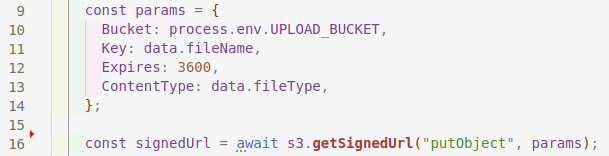
\includegraphics[width=11cm]{immagini/getURL.png} \\
		\caption{\label{fig:getURL} Snippet di codice per ottenere l'URL presigned}
	\end{figure}
	
	Nel codice sopra riportato:
	\begin{itemize}
		\item \textbf{Bucket}: nome del \emph{bucket} su cui effettuare l'operazione;
		\item \textbf{Key}: nome del file che si vuole caricare con il presigned che si ottiene, specificando eventuali prefissi;
		\item \textbf{ContentType}: tipo del file che si vuole caricare. Nel caso delle immagini caricate da MariBa è \emph{image/jpeg};
		\item \textbf{``putObject''}: tipo di operazione che si vuole effettuare con l'URL generato. In questo caso si 
		tratta di un'operazione PUT.
	\end{itemize}
	Le immagini caricate hanno utilità molto breve: infatti una volta che il back-end ne ha effettuato il download, 
	esse non verranno più utilizzate. Di conseguenza, per evitare di occupare spazio all'interno del \emph{bucket} inutilmente, è stata impostata una \emph{lifecycle rule} in modo tale che tutte le immagini (con prefisso \emph{img/}) vengano eliminate in modo automatico dopo un giorno dal loro caricamento.
	Per informazioni specifiche riguardo alla \emph{lifecycle rule} fare riferimento alla \autoref{subsec:bucketS3}.
	
	\subsubsection{AWS Lambda}
	Di seguito sono descritte le funzioni \emph{Lambda} implementate per il corretto funzionamento della funzionalità di riconoscimento automatico dei giocatori:
	\begin{itemize}
		\item \texttt{getPresignedUpload}: richiede ad \emph{S3} il presigned URL per il caricamento dell'immagine in uno specifico \emph{bucket} e con uno specifico prefisso;
		\item \texttt{callRekognition}: effettua il download dell'immagine dal \emph{bucket} S3 in modo che possa essere utilizzata da \texttt{elaborateImage};
		\item \texttt{elaborateImage}: effettua le chiamate effettive a \emph{Rekognition}. In particolare:
			\begin{enumerate}
				\item Individua i volti nella fotografia utilizzando \texttt{rekognition.DetectFaces}, la quale restituisce le relative \emph{bounding box};
				\item Ritaglia i volti individuati utilizzando tali \emph{bounding box};
				\item Per ciascun volto ritagliato chiama \texttt{rekognition.SerachFacesByImage} per cercare eventuali corrispondenze all'interno della \emph{collection} contenente tutti i volti precedentemente salvati;
				\item Se sono state trovate delle somiglianze, \texttt{rekognition.SearchFacesByImage} restituisce i \emph{faceId} corrispondenti in ordine decrescente di probabilità;
				\item Per ciascun volto individuato nell'immagine iniziale, \texttt{elaborateImage} restituisce le informazioni sulla relativa bounding box. Inoltre, nel caso fossero state trovate corrispondenze, restituisce anche il \emph{faceId}. In caso contrario restituisce invece i crop dei visi non riconosciuti.
			\end{enumerate}
		\item \texttt{updatePlayer}: aggiorna un giocatore già presente nel database con il nuovo \emph{faceId} nel momento in cui esso viene associato dall'utente;
		\item \texttt{indexFace}: utilizza \texttt{rekognition.IndexFaces} per indicizzare nuove facce all'interno della \emph{collection} di \emph{Rekognition}.
	\end{itemize}
	
	
	
	\subsection{Funzionamento generale}
	Il funzionamento generale del sistema di riconoscimento tramite immagine è schematizzato in \autoref{fig:funzionamento-rek}.
	
	\begin{figure}[H]
		\centering
		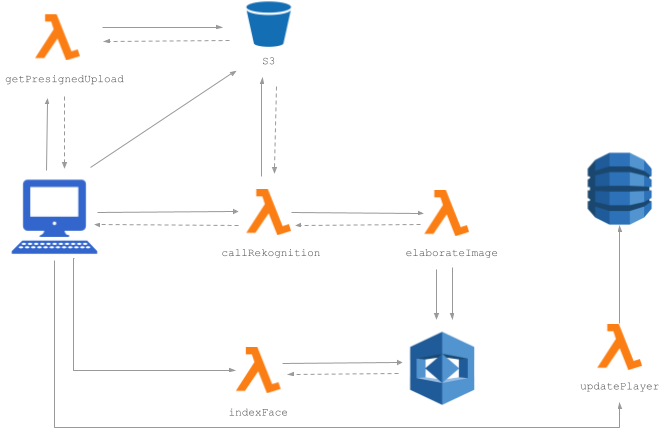
\includegraphics[width=12cm]{immagini/funzionamento.png} \\
		\caption{\label{fig:funzionamento-rek} Grafico del funzionamento del sistema di image recognition}
	\end{figure}

	In particolare avvengono le seguenti operazioni:
	\begin{itemize}
		\item Il front-end utilizza la funzione \texttt{getPresignedUpload} per ottenere l'URL per il caricamento dell'immagine nel \emph{bucket} \emph{S3};
		\item Una volta ottenuto il link, il front-end procede al caricamento;
		\item Chiama la funzione \texttt{callRekognition} e attende i dati delle facce individuate e/o riconosciute;
		\item \texttt{callRekognition} scarica l'immagine dal \emph{bucket} e la passa a \texttt{elaborateImage};
		\item \texttt{elaborateImage} esegue le chiamate effettive a \emph{Rekognition} come descritte nella \autoref{subsec:rekognition};
		\item \texttt{elaborateImage} ritorna il risultato dell'elaborazione opportunamente strutturato a \texttt{callRekognition} che a sua volta lo restituisce al front-end;
		\item Il front-end visualizza i dati ricevuti;
		
		\item Se viene richiesto di registrare un nuovo utente:
		\begin{itemize}
			\item Viene chiamata \texttt{indexFace} per indicizzare il crop del viso non ancora registrato nella \emph{collection} di \emph{Rekognition};
			\item \texttt{indexFace} restituisce il \emph{faceId} del viso indicizzato; 
			\item Viene aggiunto un nuovo record nel database contenente le informazioni del nuovo giocatore, compreso il \emph{faceId} ricevuto;
		\end{itemize}
		
		\item Se viene richiesto di associare un nickname già esistente ad un viso:
		\begin{itemize}
				\item Viene chiamata \texttt{indexFace} per indicizzare il crop del viso non ancora registrato nella \emph{collection} di \emph{Rekognition};
			\item \texttt{indexFace} restituisce il \emph{faceId} del viso indicizzato; 
			\item Viene chiamata \texttt{updatePlayer} per inserire il \emph{faceId} nel record del giocatore da associare. Nel caso in cui vi fosse già un \emph{faceId}, questo viene sostituito.
		\end{itemize}
		
	\end{itemize}
	
		
		
	
	
	\subsection{Design dell'interfaccia}
	Per il design dell'interfaccia, prima della sua effettiva codifica, sono stati realizzati dei \emph{wireframes} utilizzando \emph{Balsamiq}. In questo modo si è potuto definire il flusso di funzionamento a livello di front-end. \\ 

	\noindent Successivamente, lo sviluppo dell'interfaccia è avvenuto utilizzando \emph{Angular 12.x} in collaborazione con la libreria 
	\emph{Nebular}, specifica per la creazione di interfacce utente. \\
	
	\noindent Nei paragrafi seguenti viene mostrata l'interfaccia realizzata per l'inserimento dei giocatori attraverso l'utilizzo della funzionalità di riconoscimento.
	
		\subsubsection{Inserimento di una nuova partita di calcetto}
		Nella pagina per l'inizializzazione di una nuova partita di calcetto è stato aggiunto un pulsante per attivare la webcam e scattare la foto  contenente i volti dei giocatori (\autoref{fig:calcetto-1}). Lo scatto viene quindi inviato a \emph{Amazon Rekognition} per effettuare il riconoscimento facciale. 
		
		\begin{figure}[H]
			\centering
			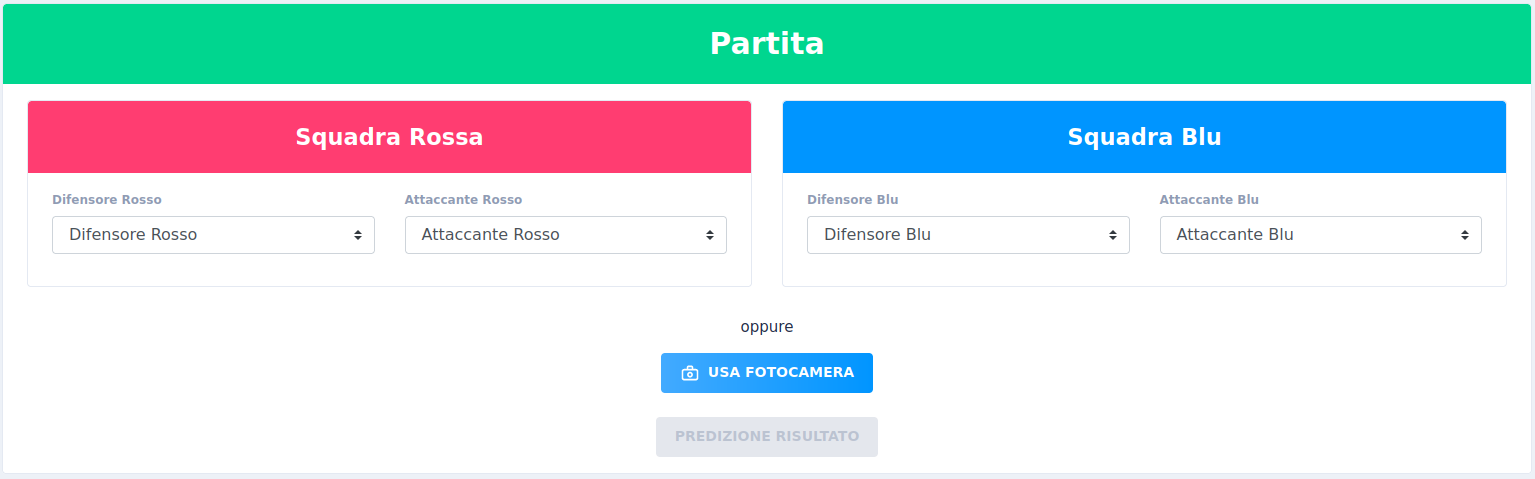
\includegraphics[width=\textwidth]{immagini/calcetto-1.png} \\
			\caption{\label{fig:calcetto-1} Schermata iniziale di calcetto}
		\end{figure}
	
		\noindent Una volta ricevuto il risultato dell'elaborazione, i giocatori vengono visualizzati in card selezionabili per la formazione delle squadre (\autoref{fig:calcetto-2}). I giocatori possono appartenere a tre categorie differenti:
		\begin{itemize}
			\item \textbf{Giocatore riconosciuto}: viene mostrato il nickname corrispondente al volto riconosciuto;
			\item \textbf{Giocatore non riconosciuto ma registrato}: il giocatore è già registrato ma non ha ancora un volto associato. Quando selezionato richiede l'associazione del nickname al viso scegliendo tra i nickname già presenti nel database;  
			\item\textbf{Giocatore non riconosciuto e non registrato}: quando selezionato richiede la registrazione di un nuovo giocatore; 
		\end{itemize}
	
		\noindent Nel caso in cui uno o più giocatori partecipanti non fossero presenti all'interno della fotografia scattata o non fossero stati individuati, è possibile inserirli manualmente: premendo sull'apposito pulsante viene mostrato un pop-up nel quale selezionare il nickname del giocatore da aggiungere. Una volta confermato l'inserimento, viene mostrata la card corrispondente. \\
		Il numero di giocatori selezionabili per ciascuna squadra è esattamente due. 
		
		\begin{figure}[H]
			\centering
			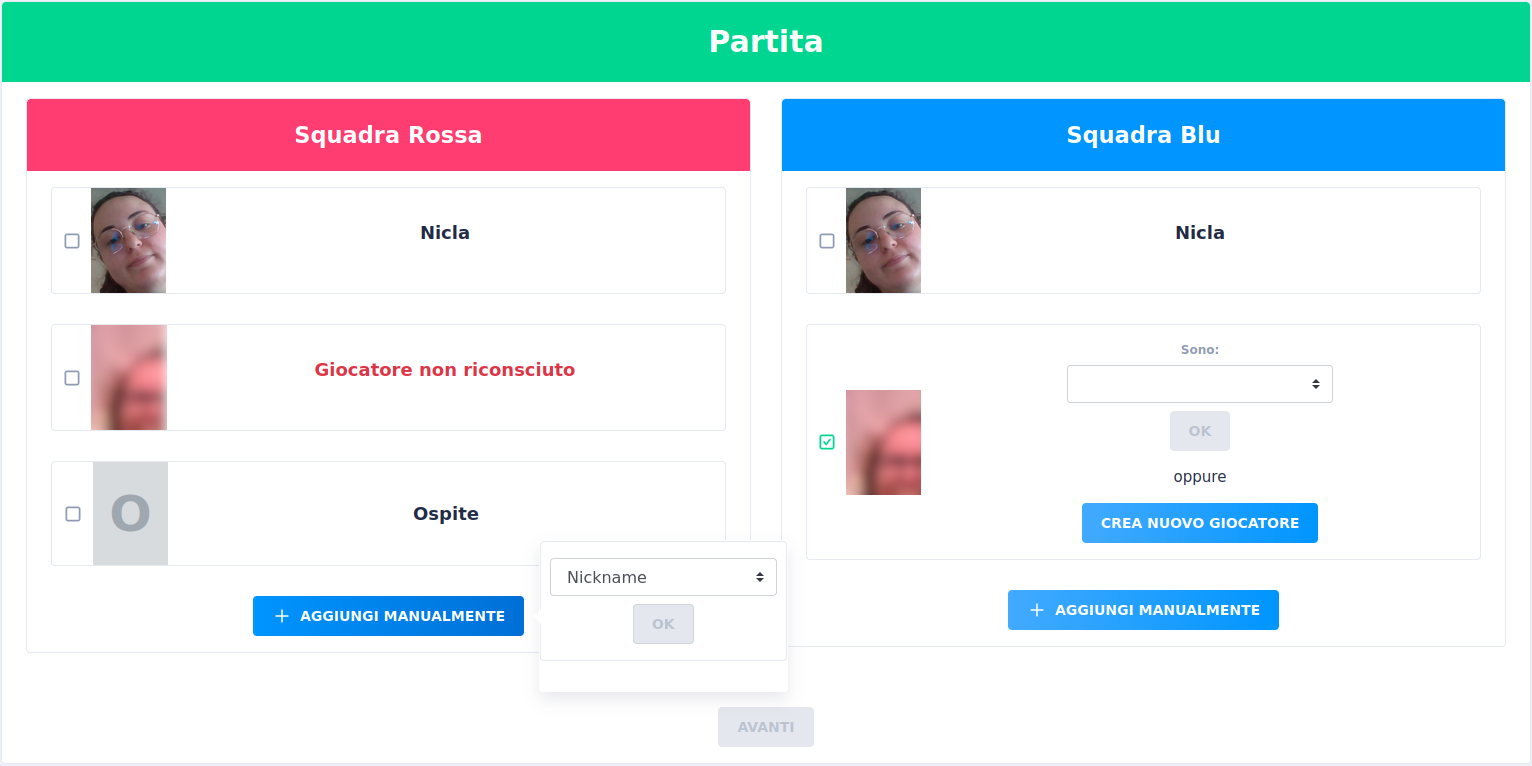
\includegraphics[width=\textwidth]{immagini/calcetto-2.png} \\
			\caption{\label{fig:calcetto-2} Selezione dei giocatori}
		\end{figure}
		
		\noindent Dopo la selezione dei giocatori sarà infine possibile scambiare i due nickname all'interno di ciascuna squadra per associare loro il ruolo desiderato e creare la formazione definitiva (\autoref{fig:calcetto-3}).
			
		\begin{figure}[H]
			\centering
			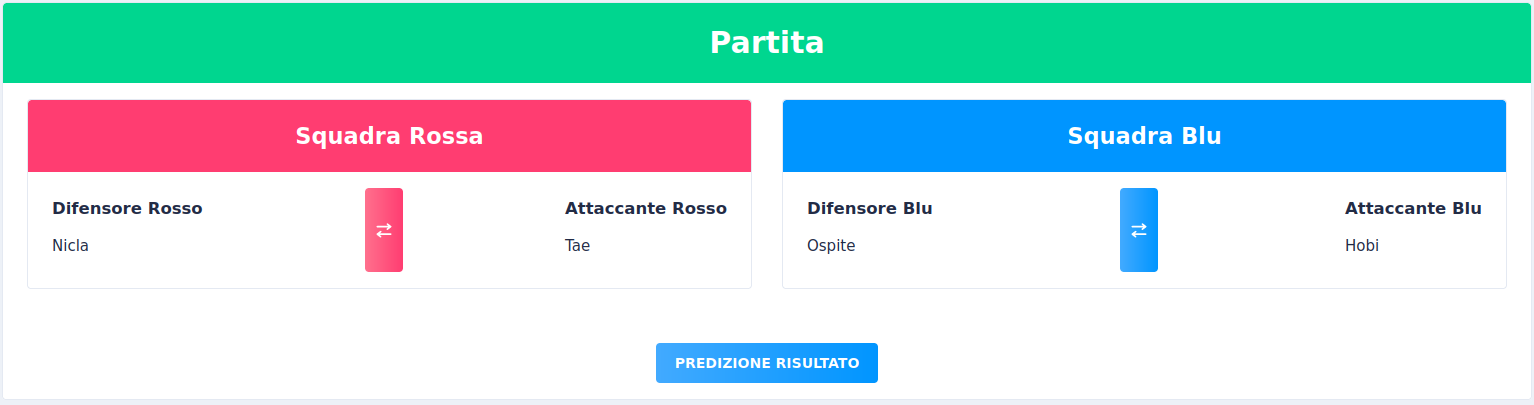
\includegraphics[width=\textwidth]{immagini/calcetto-3.png} \\
			\caption{\label{fig:calcetto-3} Formazione squadre di calcetto}
		\end{figure}
		
		
		\subsubsection{Inserimento di una nuova partita di Mario Kart e Duck Game}
		Il procedimento da seguire per l'inserimento di una partita di Mario Kart o di Duck Game tramite l'utilizzo del riconoscimento facciale dei giocatori è pressoché il medesimo. \\
		La sola differenza tra i due giochi è individuabile nel numero di giocatori selezionabili: 
		\begin{itemize}
			\item per Mario Kart devono essere inseriti esattamente quattro giocatori (\autoref{fig:kart-1});
			\item per Duck Game si possono inserire da un minimo di due ad un massimo di otto giocatori (\autoref{fig:duck-1}).
		\end{itemize}
	
		Ad entrambe le schermate, come per calcetto, è stato quindi aggiunto un pulsante per attivare la webcam e scattare la fotografia da inviare ad \emph{Amazon Rekognition}.
		
		\begin{figure}[H]
			\centering
			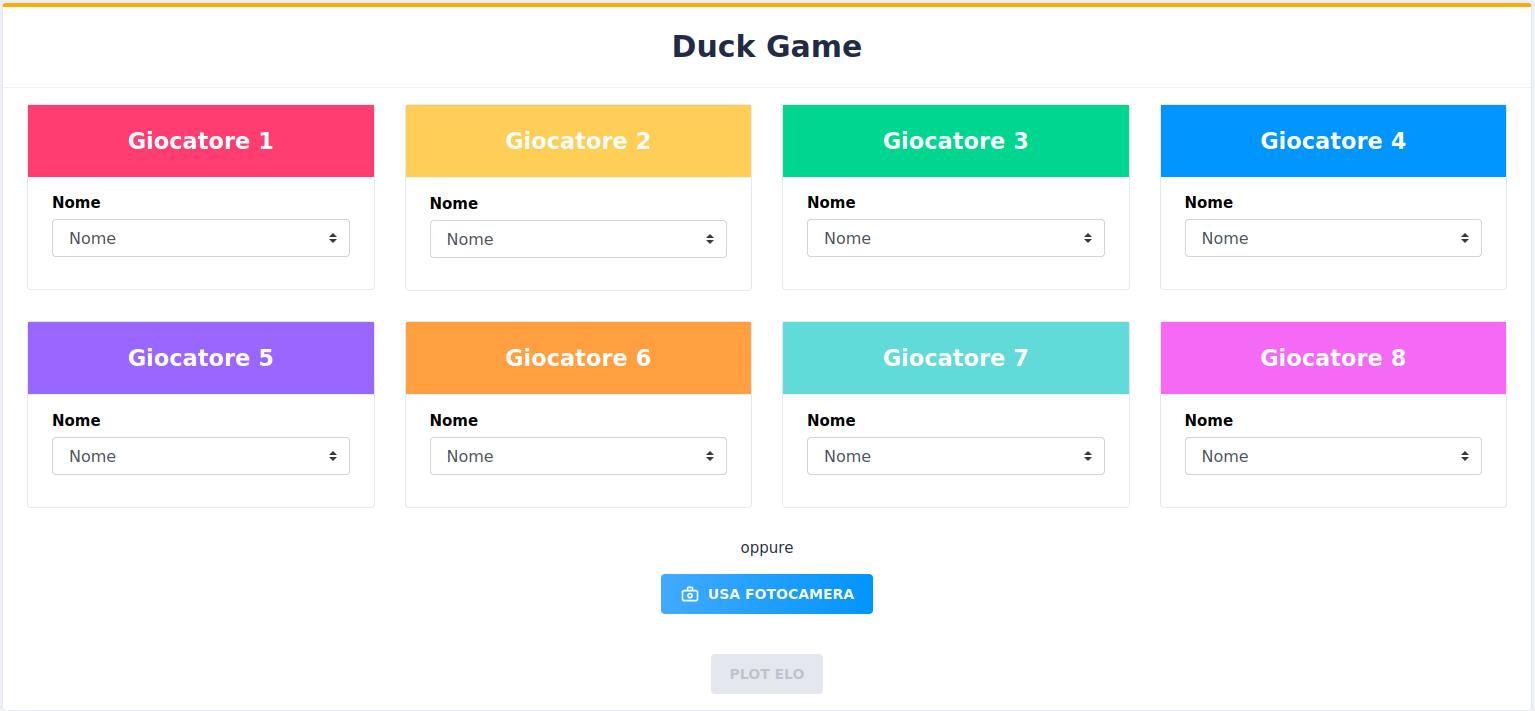
\includegraphics[width=\textwidth]{immagini/duck-1.png} \\
			\caption{\label{fig:duck-1} Schermata iniziale di Duck Game}
		\end{figure}
	
		\begin{figure}[H]
			\centering
			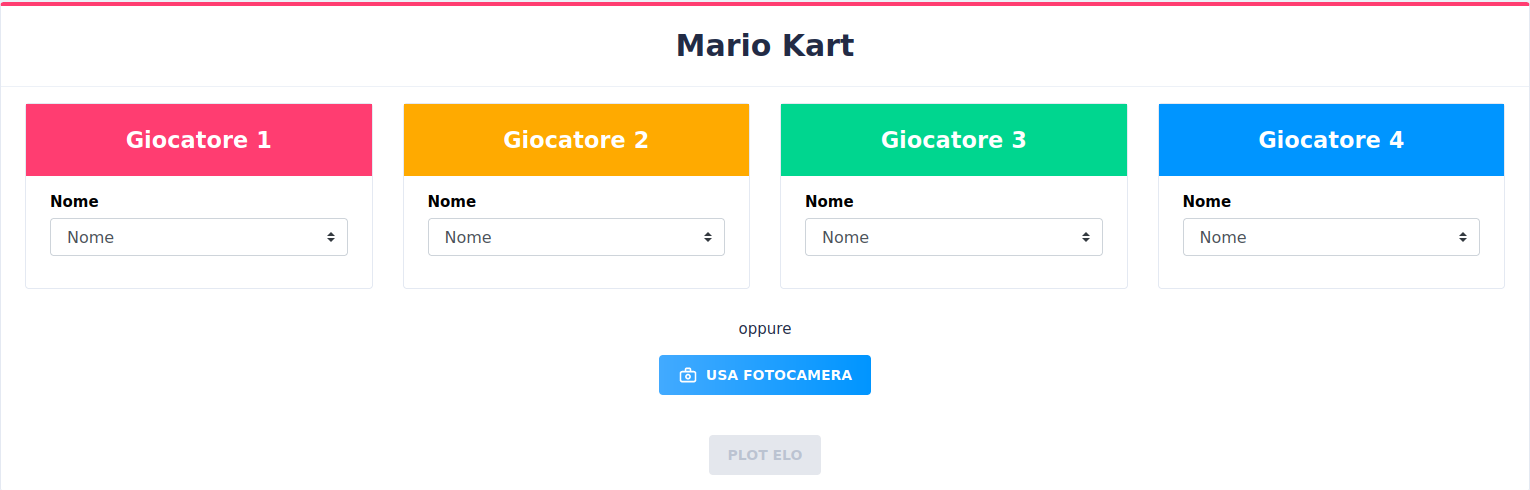
\includegraphics[width=\textwidth]{immagini/kart-1.png} \\
			\caption{\label{fig:kart-1} Schermata iniziale di Mario Kart}
		\end{figure}
		
		\noindent Una volta ricevuto il risultato dell'elaborazione, i giocatori vengono visualizzati in card selezionabili (\autoref{fig:kart-2}). I giocatori possono appartenere a tre categorie differenti:
		\begin{itemize}
			\item \textbf{Giocatore riconosciuto}: viene mostrato il nickname corrispondente al volto riconosciuto;
			\item \textbf{Giocatore non riconosciuto ma registrato}: il giocatore è già registrato ma non ha ancora volto associato. Quando selezionato richiede l'associazione del nickname al viso scegliendo tra i nickname già presenti nel database; 
			\item\textbf{Giocatore non riconosciuto e non registrato}: quando selezionato richiede la registrazione di un nuovo giocatore; 
		\end{itemize} 
	
		\noindent Nel caso in cui uno o più giocatori partecipanti non fossero presenti all'interno della fotografia scattata o non fossero stati individuati, è possibile inserirli manualmente: premendo sull'apposito pulsante viene mostrato un pop-up nel quale selezionare il nickname del giocatore da aggiungere. Una volta confermato l'inserimento, viene mostrata la card corrispondente. \\
		
		\begin{figure}[H]
			\centering
			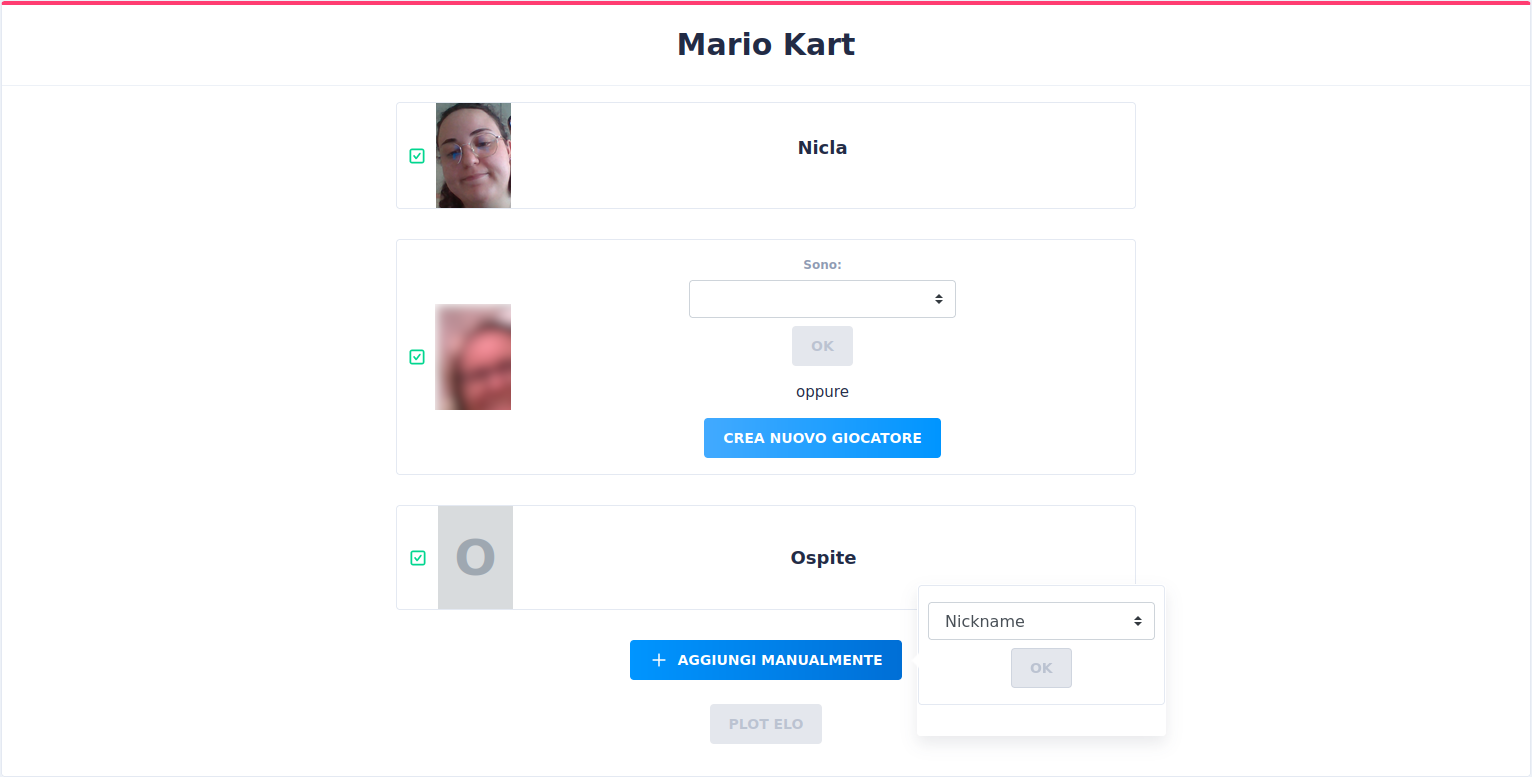
\includegraphics[width=\textwidth]{immagini/kart-2.png} \\
			\caption{\label{fig:kart-2} Selezione dei giocatori di Mario Kart}
		\end{figure}
	
		
